%% LyX 2.0.3 created this file.  For more info, see http://www.lyx.org/.
%% Do not edit unless you really know what you are doing.
\documentclass[10pt,spanish]{article}
\usepackage[utf8x]{inputenc}
\usepackage[letterpaper]{geometry}
\geometry{verbose}
\usepackage{amsmath}
\usepackage{amssymb}
\usepackage{graphicx}

\makeatletter

%%%%%%%%%%%%%%%%%%%%%%%%%%%%%% LyX specific LaTeX commands.
%% A simple dot to overcome graphicx limitations
\newcommand{\lyxdot}{.}


%%%%%%%%%%%%%%%%%%%%%%%%%%%%%% User specified LaTeX commands.

\usepackage{ucs}\usepackage[spanish]{babel}
\usepackage{amsfonts}\usepackage{colortbl}% = = = = = = = = = = = = = = = = = = = = = = = = =
% INICIO EL DOCUMENTO
% = = = = = = = = = = = = = = = = = = = = = = = = =



\usepackage{babel}
\addto\shorthandsspanish{\spanishdeactivate{~<>}}





\usepackage{babel}
\addto\shorthandsspanish{\spanishdeactivate{~<>}}



\usepackage{babel}
\addto\shorthandsspanish{\spanishdeactivate{~<>}}





\usepackage{babel}
\addto\shorthandsspanish{\spanishdeactivate{~<>}}





\usepackage{babel}
\addto\shorthandsspanish{\spanishdeactivate{~<>}}





\usepackage{babel}
\addto\shorthandsspanish{\spanishdeactivate{~<>}}





\usepackage{babel}
\addto\shorthandsspanish{\spanishdeactivate{~<>}}





\usepackage{babel}
\addto\shorthandsspanish{\spanishdeactivate{~<>}}





\usepackage{babel}
\addto\shorthandsspanish{\spanishdeactivate{~<>}}



\usepackage{babel}
\addto\shorthandsspanish{\spanishdeactivate{~<>}}





\usepackage{babel}
\addto\shorthandsspanish{\spanishdeactivate{~<>}}





\usepackage{babel}
\addto\shorthandsspanish{\spanishdeactivate{~<>}}





\usepackage{babel}
\addto\shorthandsspanish{\spanishdeactivate{~<>}}





\usepackage{babel}
\addto\shorthandsspanish{\spanishdeactivate{~<>}}





\usepackage{babel}
\addto\shorthandsspanish{\spanishdeactivate{~<>}}





\usepackage{babel}
\addto\shorthandsspanish{\spanishdeactivate{~<>}}

\makeatother

\usepackage{babel}
\addto\shorthandsspanish{\spanishdeactivate{~<>}}

\begin{document}

\section{Pantallas Generales}

\label{sec:PG}


\subsection{PG1 Iniciar Sesión}

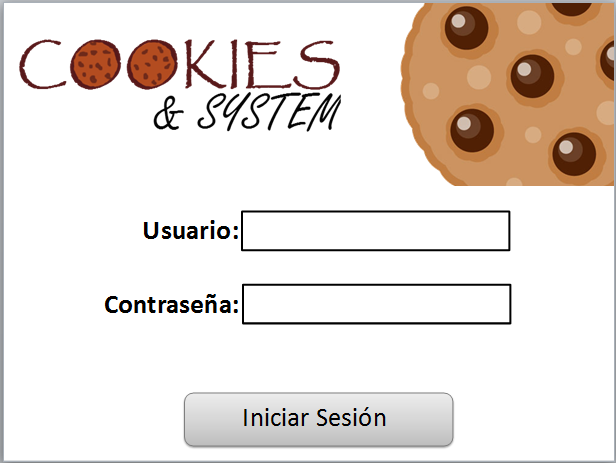
\includegraphics{PG1}


\subsection{PG2 Notificaciones}

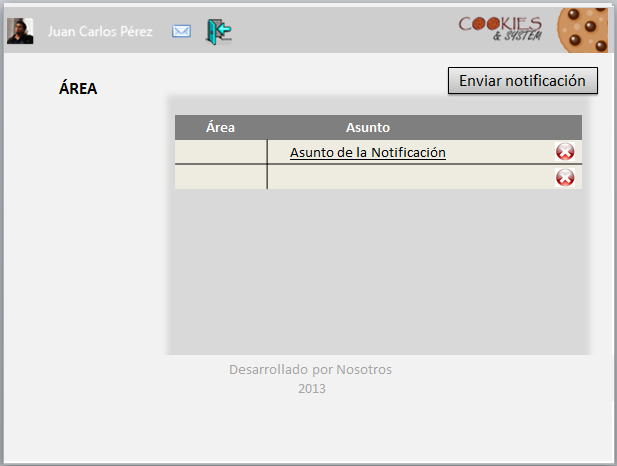
\includegraphics{PG2}


\subsection{PG3 Enviar notificación}

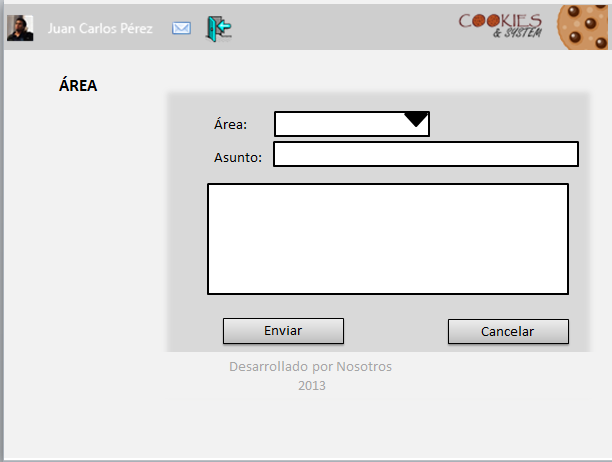
\includegraphics{PG3}


\subsection{PG4 Visualizar notificación}

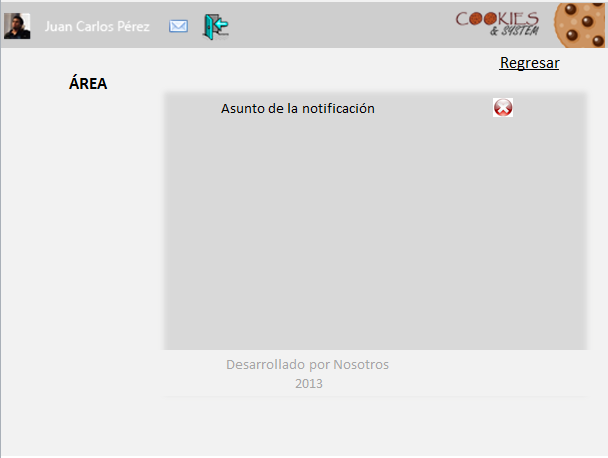
\includegraphics{PG4}


\section{Pantallas Administrador}

\label{sec:PA}


\subsection{PA0 Inicio del administrador}

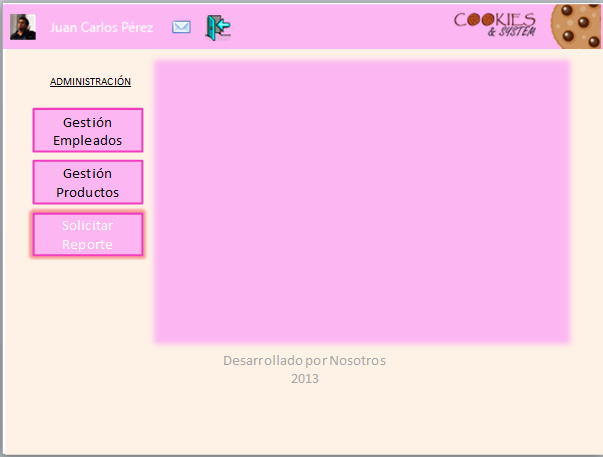
\includegraphics{PA0}


\subsection{PA1 Gestión de productos}

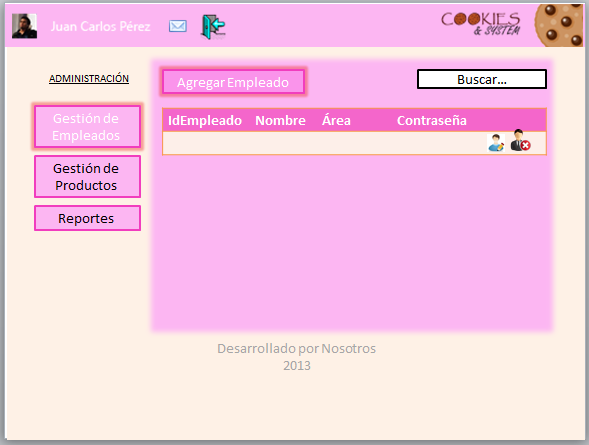
\includegraphics{PA1}


\subsection{PA2 Registrar Producto}

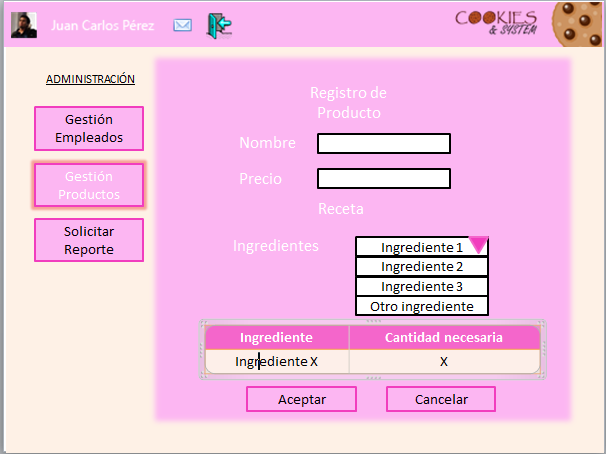
\includegraphics{PA2}


\subsection{PA3 Modificar Producto}

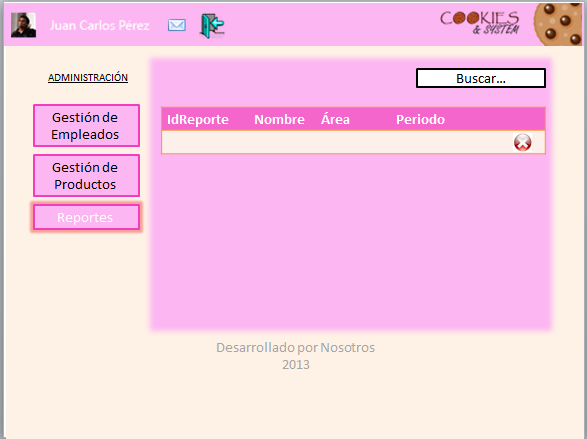
\includegraphics{PA3}


\subsection{PA4 Gestión de Empleados}

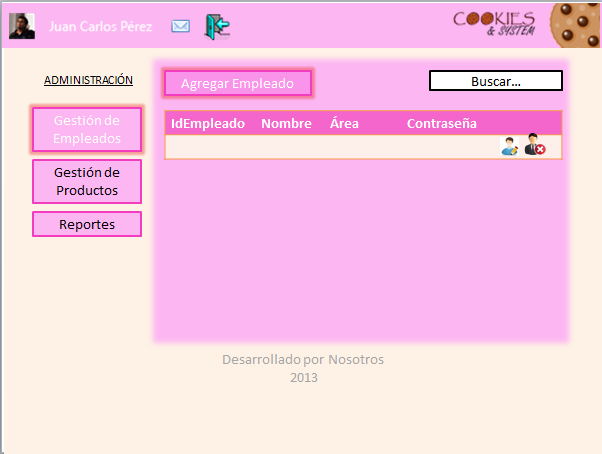
\includegraphics{PA4}


\subsection{PA5 Registrar Empleado}

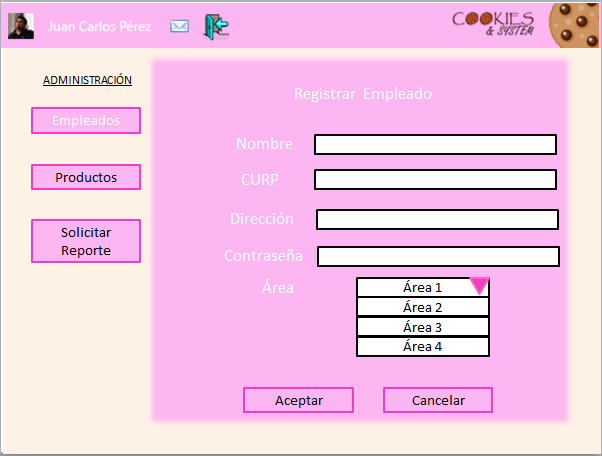
\includegraphics{PA5}


\subsection{PA6 Modificar Empleado}

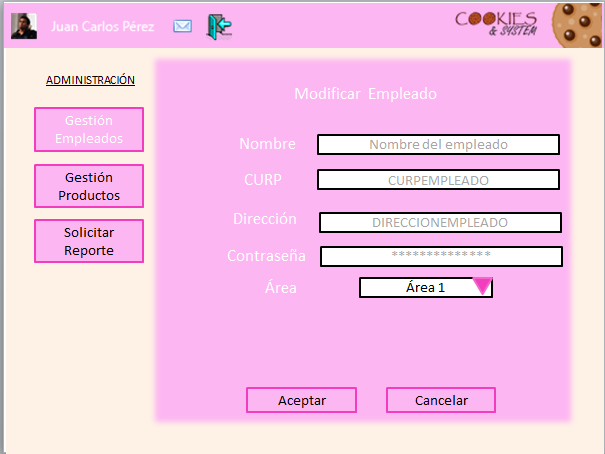
\includegraphics{PA6}


\subsection{PA7 Reportes}

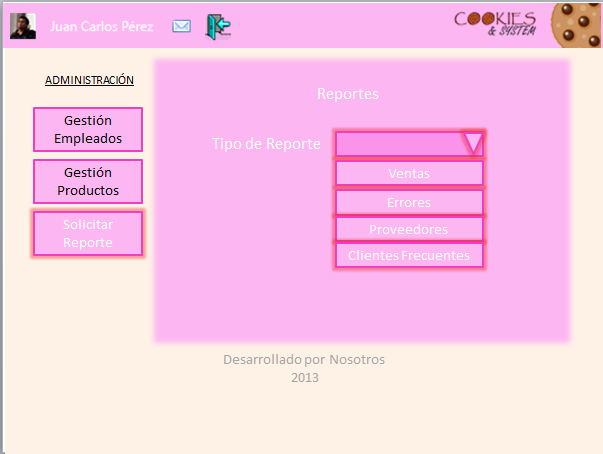
\includegraphics{PA7}


\section{Pantallas Control de Calidad.}

\label{sec:PCC}


\subsection{PCC1 Visualiza Problemas}

\includegraphics{PCC1\lyxdot 1}


\subsection{PCC2 Detalles del Problema}

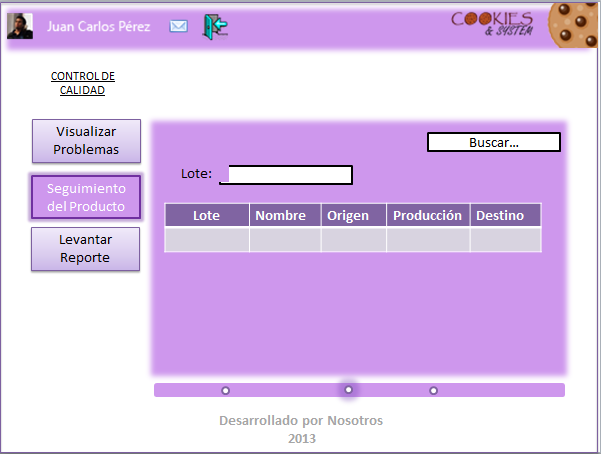
\includegraphics{PCC2}


\subsection{PCC3 Seguimiento del Producto.}

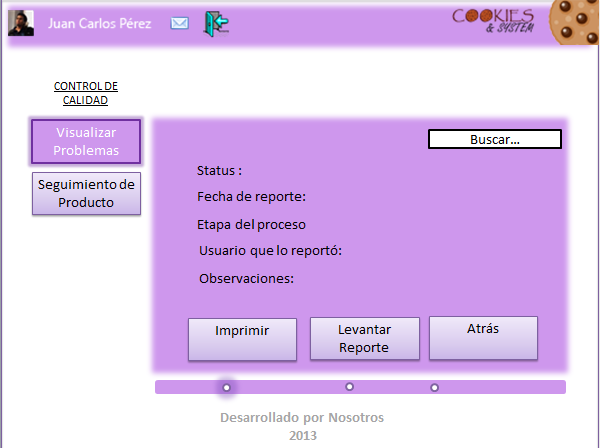
\includegraphics{PCC3}


\section{Pantallas Ventas}


\subsection{PV4.1 Registrar Venta}

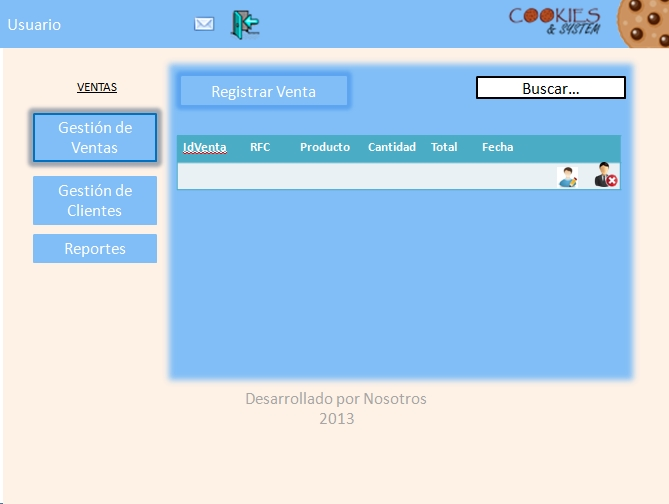
\includegraphics[scale=0.75]{PV1}


\subsection{PV4.1 Registrar Pedido}

\includegraphics[scale=0.75]{pv11}


\subsection{PV5.0 Modificar Venta}

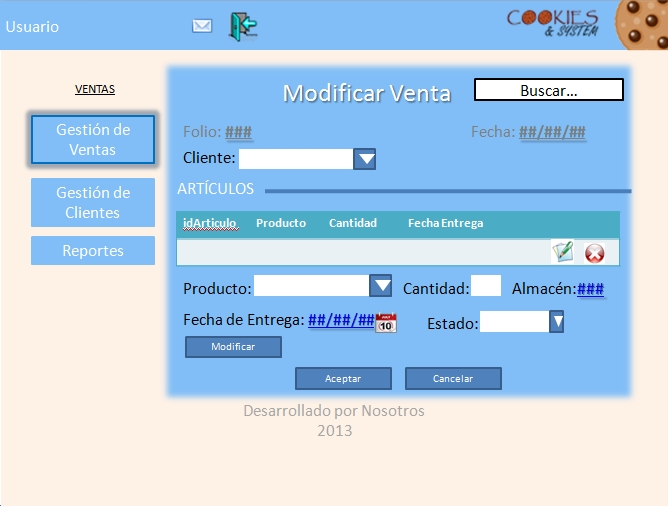
\includegraphics[scale=0.75]{PV12}


\subsection{PV5.1 Gestión de clientes}

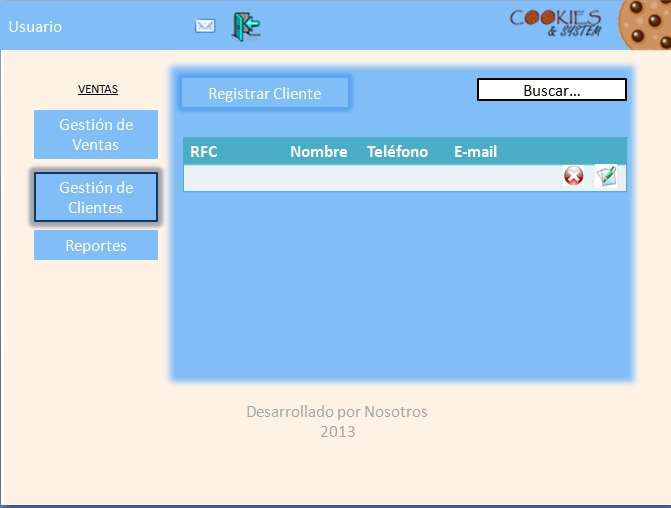
\includegraphics{PV2}


\subsection{PV5.2 Agregar cliente}

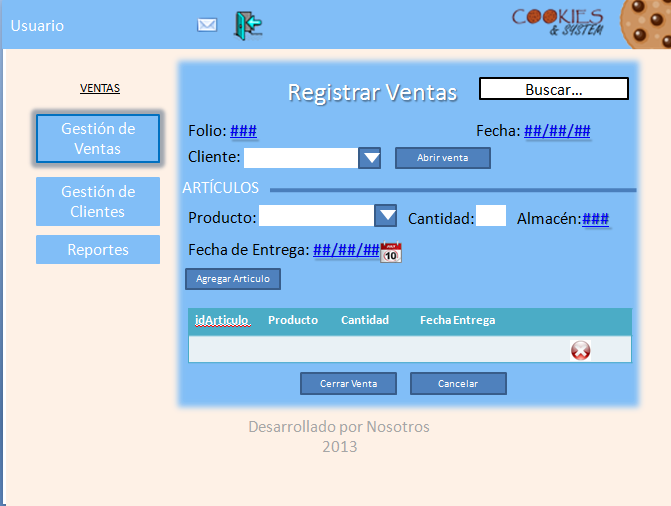
\includegraphics[scale=0.75]{PV21}


\subsection{PV5.3 Modificar Cliente}

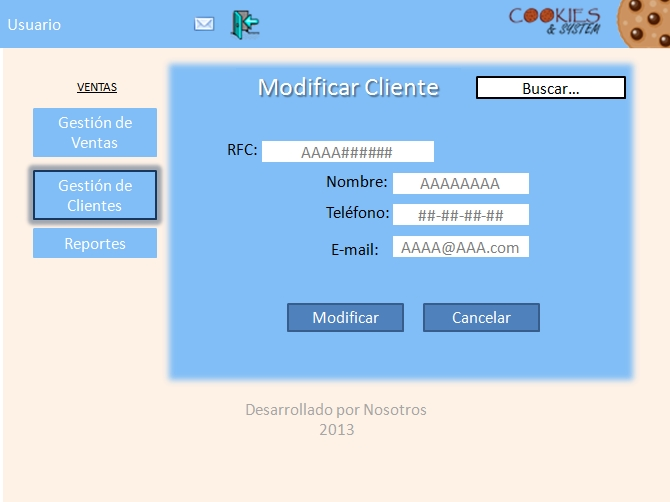
\includegraphics[scale=0.75]{PV22}


\section{Pantallas Compras.}


\subsection{PC1 Gestión Proveedores}

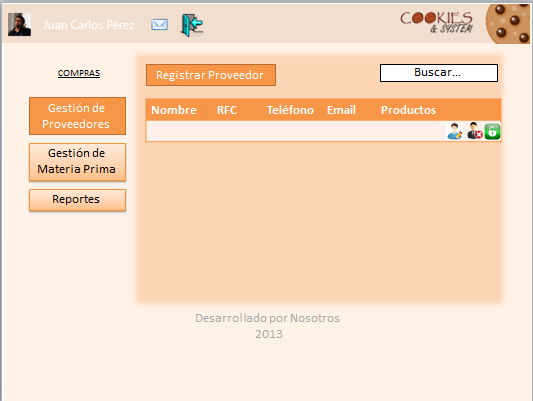
\includegraphics{PC1}


\subsection{PC2 Gestión de materia prima}

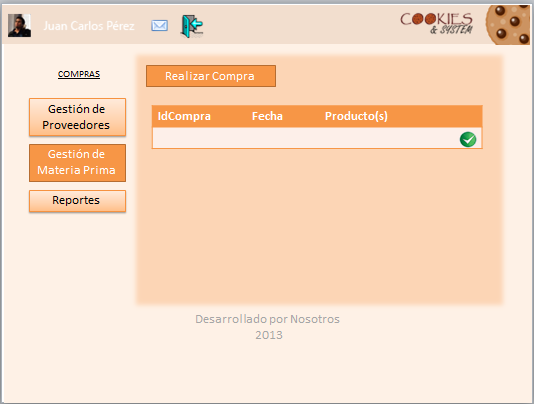
\includegraphics{PC2}


\subsection{PC3 Realizar compra}

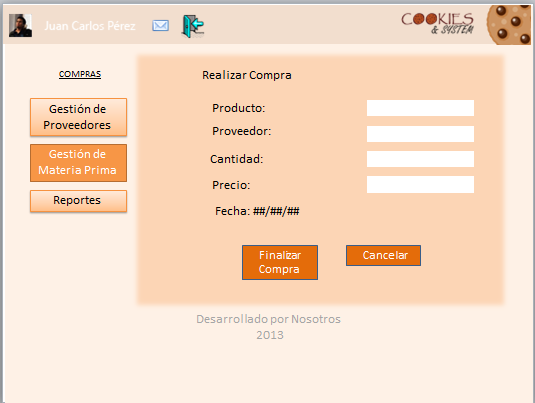
\includegraphics{PC3}


\subsection{PC4 Reportes}

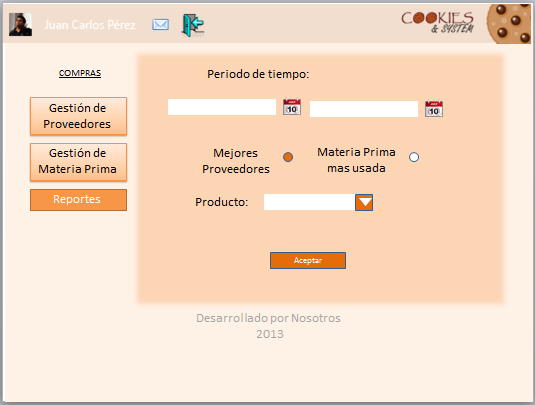
\includegraphics{PC4}


\subsection{PC5 Registrar Proveedor.}

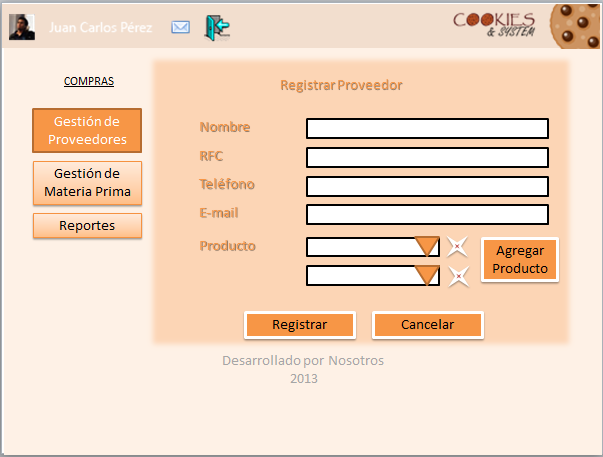
\includegraphics{PC5}


\subsection{PC6 Modificar Proveedor}

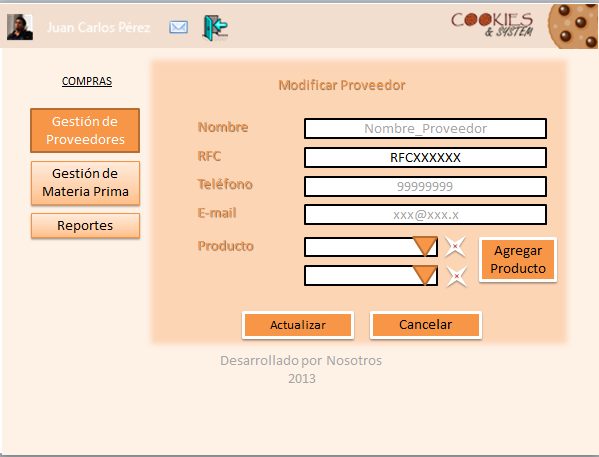
\includegraphics{PC6}


\section{Pantallas Inventarios.}


\subsection{PI1 Inicio Inventario}

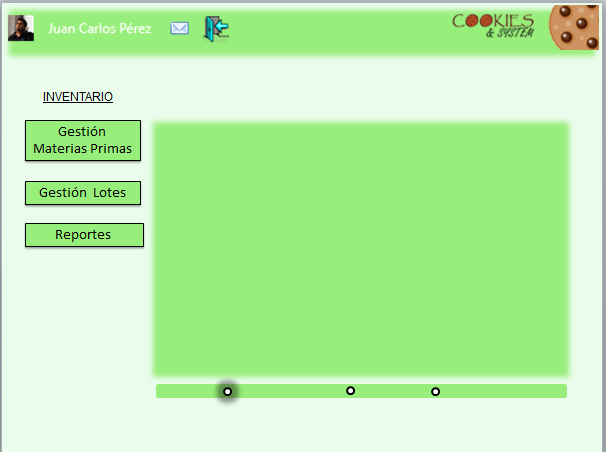
\includegraphics{PI1}


\subsection{PI2 Gestión Materias Primas}

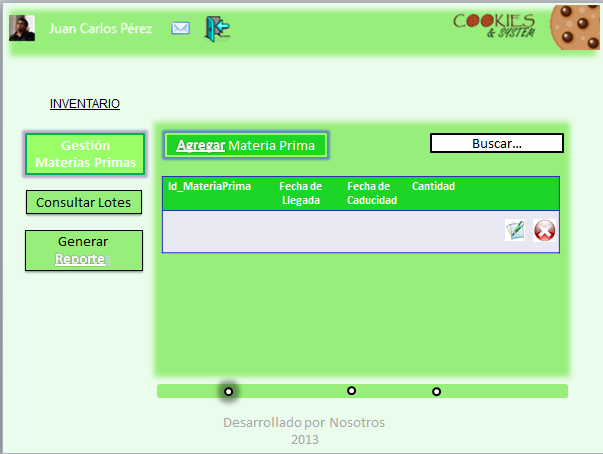
\includegraphics{PI2}


\subsection{PI3 Consultar Lotes}

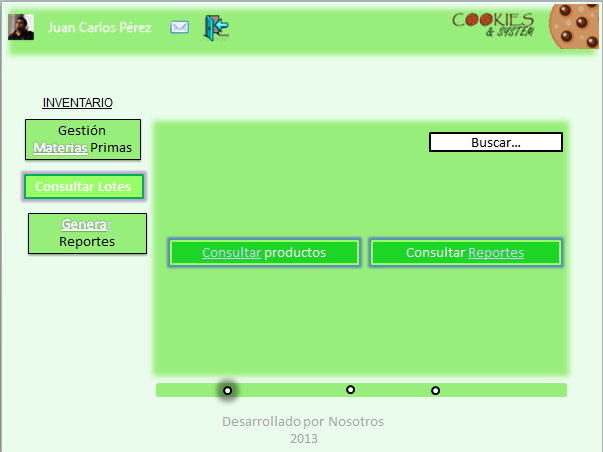
\includegraphics{PI3}


\subsection{PI4 Generar reportes}

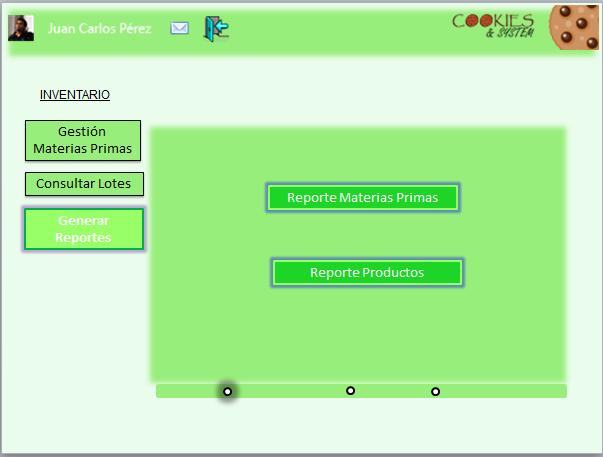
\includegraphics{PI4}


\subsection{PI5 }

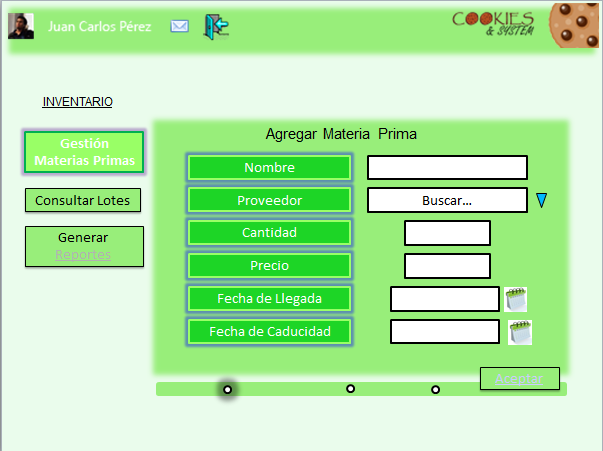
\includegraphics{PI5}


\subsection{PI6 Consultar productos}

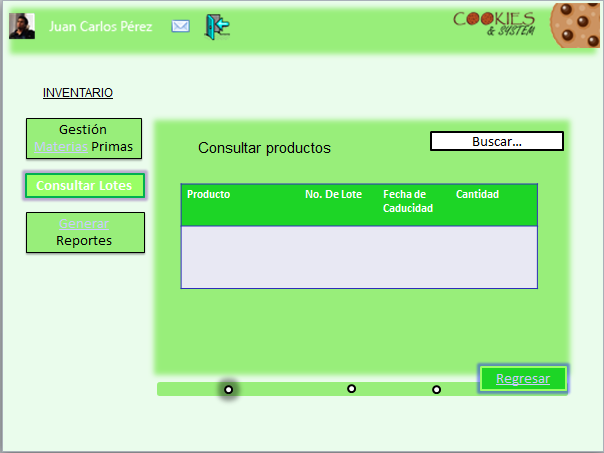
\includegraphics{PI6}


\subsection{PI7 Consultar reportes}

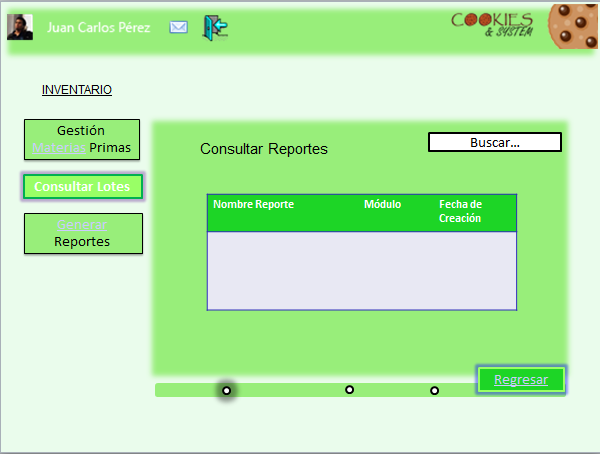
\includegraphics{PI7}


\section{Pantallas Producción.}


\subsection{PP1 Consultar estado del almacen}

\includegraphics[scale=0.5]{MenuProduccionNuevo}


\subsection{PP2 Consultar pedidos en espera}

\includegraphics[scale=0.5]{MenuProduccionNuevo2}


\subsection{PP3 Consultar disponibilidad de ingredientes}

\includegraphics[scale=0.5]{MenuProduccionNuevo3}


\subsection{PP4 Asigar líneas de producción}

\includegraphics[scale=0.5]{MenuProduccionNuevo4}


\subsection{PP5 Gestionar lotes}

\includegraphics[scale=0.5]{MenuProduccionNuevo5}


\subsection{PP6 Registrar lote}

\includegraphics[scale=0.5]{MenuProduccionNuevo6}


\subsection{PP7 Consultar lote}

\includegraphics[scale=0.5]{MenuProduccionNuevo7}
\end{document}
